\documentclass{beamer}
\usepackage[utf8]{inputenc}
\usepackage{url}
\usepackage{hyperref}
\graphicspath{{./fig/aula7}}

% Configurando layout para mostrar codigos C++
\usepackage{listings}
\lstset{
  language=HTML,
  basicstyle=\ttfamily\small, 
  keywordstyle=\color{blue}, 
  stringstyle=\color{red}, 
  commentstyle=\color{red}, 
  extendedchars=true, 
  showspaces=false, 
  showstringspaces=false, 
  numbers=left,
  numberstyle=\tiny,
  breaklines=true, 
  backgroundcolor=\color{green!10},
  breakautoindent=true, 
  captionpos=b,
  xleftmargin=0pt,
}
date{}

\title{Desenvolvimento Web Básico}
\subtitle{Aula 9}

\usetheme{lucid}

\begin{document}
\frame{
 \titlepage
}

%--------------------------------------------------------------------------
\begin{frame}{Na aula de hoje...} 
\tableofcontents 
\end{frame}

%--------------------------------------
\section{Formulários}
\begin{frame}{Formulários}
  \begin{enumerate}
      \item Formulários são utilizados na maior parte das aplicações Web para coletar dados dos usuários e registrar alterações nos mesmos;
      \item Vamos rever os principais elementos de formulários, e como utiliza-los com JavaScript;
  \end{enumerate}
\end{frame}
%--------------------------------------
\begin{frame}{ Eventos de Formulários}
  \begin{enumerate}
      \item Como capturar se um radio foi selecionado?
      \item Como verificar as checked box?
      \item como saber qual option de uma select foi escolhida?
  \end{enumerate}
\end{frame}
%--------------------------------------
\begin{frame}{Radio e JavaScript}
Como capturar se um radio foi selecionado?\\
Geralemnte existem vários botões de radio em uma página, para garantir a seleção única possuem apenas um \textit{name}. Como no exemplo:
\begin{center}
    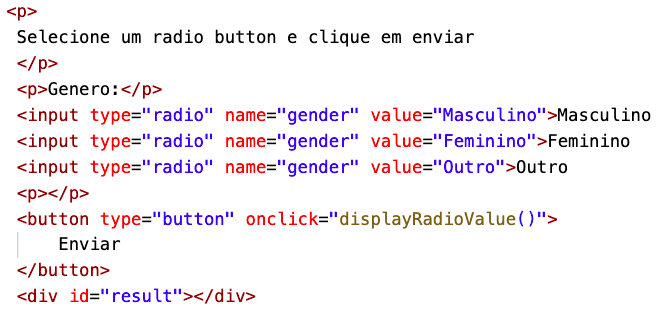
\includegraphics[height=0.5\paperheight]{fig/aula7/aula7_1.png}
\end{center}

\end{frame}
%--------------------------------------
\begin{frame}{Radio e JavaScript}
Como capturar se um radio foi selecionado?\\
Utilizando o HTML anterior, vamos coletar um array de elementos radio (por nome) e verificar qual foi selecionado, com a função \textit{checked}
\begin{center}
    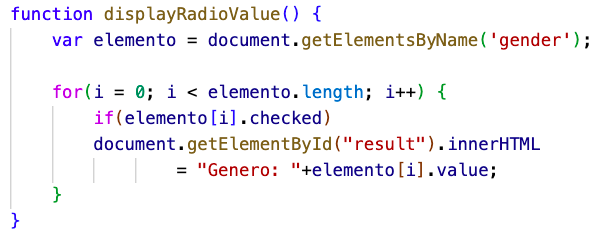
\includegraphics[height=0.4\paperheight]{fig/aula7/aula7_2.png}
\end{center}

\end{frame}
%--------------------------------------
\begin{frame}{Select e JavaScript}
Como capturar qual elemento de uma lista foi selecionado?\\
Geralmente existem vários elementos em uma lista. Como no exemplo:
\begin{center}
    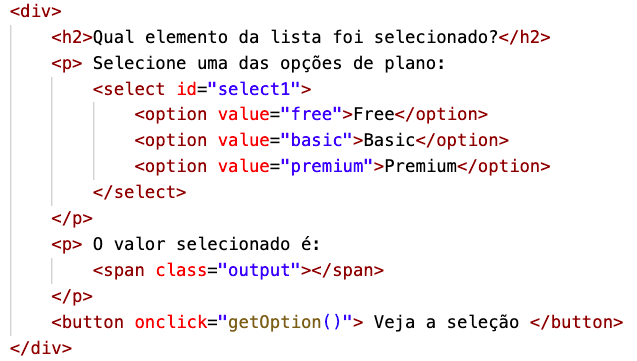
\includegraphics[height=0.5\paperheight]{fig/aula7/aula7_3.png}
\end{center}

\end{frame}
%--------------------------------------
\begin{frame}{Select e JavaScript}
Como capturar qual elemento de uma lista foi selecionado?\\
Utilizando o HTML anterior, vamos coletar o valor do elemento selecionado, utilizando querySelector(por id), e extraindo o \textit{value} do elemento;
\begin{center}
    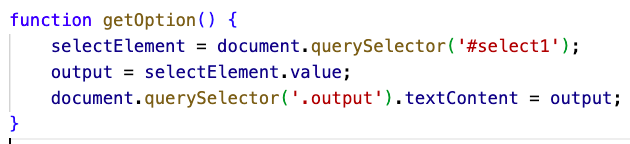
\includegraphics[height=0.25\paperheight]{fig/aula7/aula7_4.png}
\end{center}

\end{frame}
%--------------------------------------
\begin{frame}{CheckBox e JavaScript}
Como capturar quais elementos check foram selecionados?\\
Geralmente existem vários elementos check. Como no exemplo:
\begin{center}
    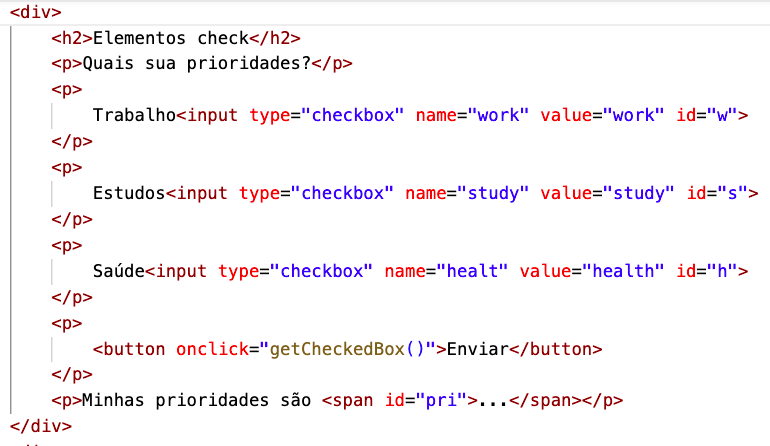
\includegraphics[height=0.5\paperheight]{fig/aula7/aula7_5.png}
\end{center}

\end{frame}
%--------------------------------------
\begin{frame}{CheckBox e JavaScript}
Como capturar quais elementos check foram selecionados?\\
Utilizando o HTML anterior, vamos coletar um array de elementos selecionador, utilizando querySelector(por tipo de input e condição), e extraindo o \textit{value} do elemento;
\begin{center}
    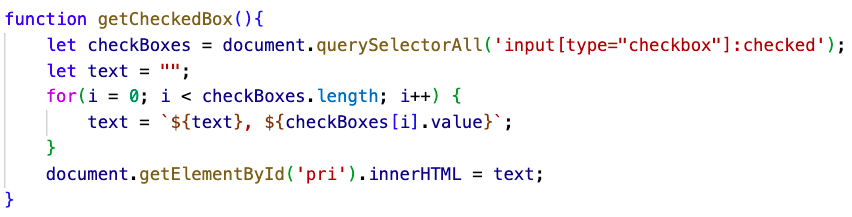
\includegraphics[height=0.25\paperheight]{fig/aula7/aula7_6.png}
\end{center}

\end{frame}
%-----------------------------------------------------------------
\section{Atividade de aula}
\begin{frame}{Atividade}{Envie seu repositório feito em aula}
  \begin{enumerate}
      \item Seguindo os passos da aula, livros indicados e, a leituras recomendadas:
      \item Desenvolva um formulário de sua preferência que contenha os campos exibidos e monte um texto com as seleções do usuário.
      \item Além disso o formulário deve mudar as cores com base em combinações de seleção diferentes;
      \item Aplique CSS com Bootstrap para posicionamento e tipografia de elementos conforme a aula anterior
  \end{enumerate}


\end{frame}
%-----------------------------------------------------------------------
\section{Leitura recomendada}
\begin{frame}{Leitura complementar}
 Para mais informações sobre Git e GitHub, leia:\\
  \vspace{0.6cm}
 \begin{columns}
   \begin{column}{0.4\textwidth}
%      \textbf{Capítulo 29}\\
 \cite{githubpages2022}\\
 E\\
 \cite{beer2015github}.
   \end{column}
   \begin{column}{0.4\textwidth}
   % 
\includegraphics[height=0.7\paperheight]{introgit.jpg} \\
   \end{column}

 \end{columns}
\end{frame}

%----------------------------------------------------------------------------
\section{Referências}

\begin{frame}{Referências}%[allowframebreaks]
\small
\begin{center}
\tiny
\bibliographystyle{apalike}
\bibliography{ref_aula}
\end{center}
\end{frame}

\end{document}